\chapter{Tx beamforming}
\label{app:appendix}

In this appendix, another function of the IWR6843 is explained: Tx beamforming. This could have been a very promising solution to the multiple person vital signs estimation problem, but sadly this solution did not work as expected. However, a lot of time has been spend researching, implementing and debugging this solution, so a short summary of the development will be given, along with some pointers to where this implementation might have gone wrong.

\section{Hypothesis}
One function in the IWR6843 is Tx beamforming. This function is used to extend the range of the sensor beyond the limits during regular operation. This is achieved by making all three of the transmitting antennas work together. Each transmitting antenna has a build-in phase modulator, which can modulate the phase of the outgoing signal. Each transmitting antenna can modify its phase in such a way that the transmitting signals bundle together to form a beam. This beam has a much lower azimuth reach, but because it is directed at a specific direction it has a lot more range. This means that the range of the sensor could reach up to 150 meters away, compared to 50 meters in normal operation. Like mentioned, the azimuth reach is much lower compared to the normal operation. There is a way to achieve the normal azimuth reach, which is recording multiple radar frames at different angles with respect to the sensor, and stitching these frames together to one big radar frame. 

This is the functionality that could have been exploited for this project, the range of the sensor doesn't have to be extended, but persons have to be separated from each other. This could be done by sending a Tx beam to the person. Because of the narrow azimuth reach, only data for this person would be captured. 

So first, a normal radar image would be generated to detect the persons available in reach of the sensor. Then, the sensor would zone in on each person present, and record radar data to do the vital signs estimation on. After a certain amount of time, the sensor would switch to another person. See Figure~\ref{fig:tx_beam_theory} for a visual representation.

\begin{figure}[t]
    \centering
    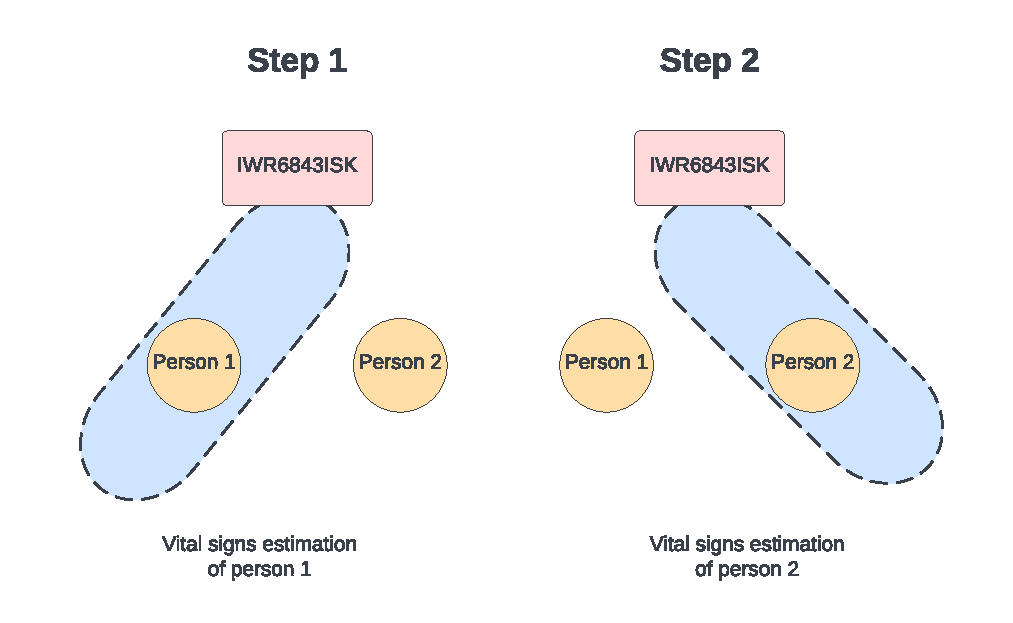
\includegraphics[width=.95\textwidth]{figures/appendix/tx_beamforming_theory2.pdf}
    \caption{The hypothesis of how the Tx beamforming would work in theory.}
    \label{fig:tx_beam_theory}
\end{figure}

\section{Implementation}
This hypothesis was implemented on the IWR6843, with the help of demo code provided by TI and the documentation available from the mmWave SDK \cite{mmwavesdk_website}. However, the SDK documentation mentioned that this feature was implemented by the developers, but there was no testing done on this feature. 

Also, when asking for help on the TI mmWave forum, they didn't have a lot of experience with this feature of the sensor. They had not tried this feature for this kind of application yet, so I wanted to give this idea a shot. I wrote a program for the IWR6843 which would form a Tx beam and steer it as much to the right as possible. The data which came back to the Rx antennae was visualized in a heatmap and send back to the computer.

\section{Results}
Sadly, this implementation did not work as expected. While the sensor was setup to steer the Tx beam all the way to the right, persons were detected in the heatmap while standing in all angles with respect to the sensor. This meant that the idea of isolating persons by Tx beamforming would not work like we expected. Even if the distance between the sensor and the person was increased to up to 4 meters, the person was detected while standing all the way to the left of the sensor. 

There are a few possible causes to this problem:

\begin{enumerate}
    \item The beam formed by the sensor could be far wider close to the sensor than expected. The real beam would only form at for example a distance of 10 meters and beyond from the sensor, which would be too much for this project. Close to the sensor the beam would look like Figure~\ref{fig:tx_beam_real_life}.
    \item Since the Tx beamforming functionality in the mmWave SDK has not been tested by the TI developers, there could be a malfunction in this technique causing it not to work properly.
    \item Because of the limited documentation, I could have implemented this functionality in the wrong way. I did extensive research on this function, but because there was almost no documentation or examples available for this function, it was mostly a case of try and error.
\end{enumerate}

In the end, it is still uncertain where the implementation of this idea went wrong. When after a lot of tries this idea still didn't work, I decided to change gears and focus on another method of getting the vital signs estimated for multiple persons at the same time. Luckily, this method did work, and you can read about all the details in the main part of this thesis.

\begin{figure}[t]
    \centering
    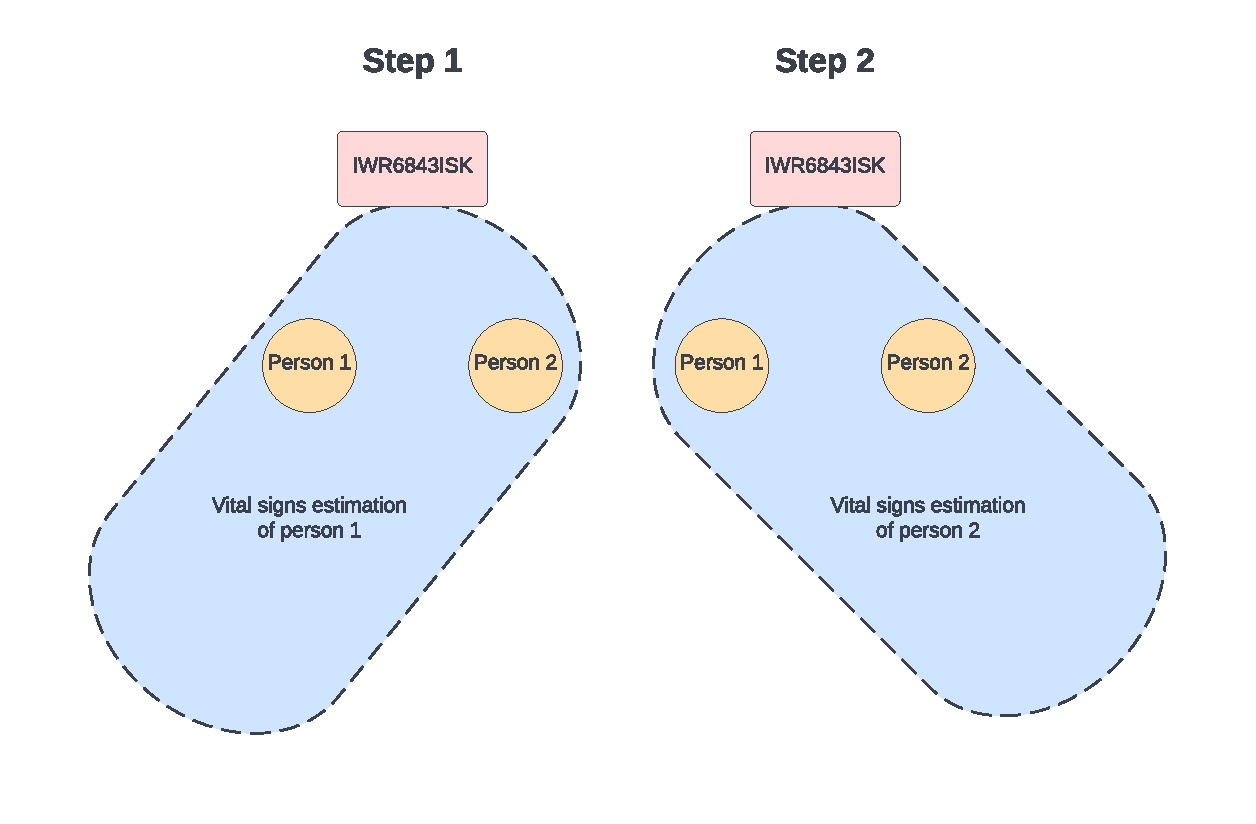
\includegraphics[width=.95\textwidth]{figures/appendix/tx_beamforming_real_life2.pdf}
    \caption{How the Tx beamforming performed during testing.}
    \label{fig:tx_beam_real_life}
\end{figure}